%%
%% Copyright (c) 2019 Weitian LI <liweitianux@sjtu.edu.cn>
%% Creative Commons BY 4.0
%%

\documentclass{beamer}

\usetheme{metropolis}
\metroset{progressbar=foot}

\setbeamertemplate{section in toc}[sections numbered]
\setbeamertemplate{frametitle continuation}{(\insertcontinuationcount)}

% Solarized theme
% Credit: https://ethanschoonover.com/solarized/
\definecolor{SolBase02}{HTML}{073642}
\definecolor{SolBase3}{HTML}{fdf6e3}
\definecolor{SolOrange}{HTML}{cb4b16}
\definecolor{SolGreen}{HTML}{859900}
%
\setbeamercolor{normal text}{fg=SolBase02, bg=SolBase3}
\setbeamercolor{alerted text}{fg=SolOrange}
\setbeamercolor{example text}{fg=SolGreen}

\setsansfont{Fira Sans Light}[
  BoldFont={Fira Sans Medium}
]
\setmonofont{Fira Code Light}[
  BoldFont={Fira Code Medium}
]

\usepackage{bm}
\usepackage{newtxsf}
\newcommand{\R}[1]{\text{#1}}  % text math alphabets
\newcommand{\Ce}{\R{e}}  % constant e
\newcommand{\Ci}{\R{i}}  % constant i
\newcommand{\Cpi}{\piup}  % upright 'pi', provided by 'newtxsf' package
\newcommand{\B}[1]{\bm{\mathsf{#1}}}  % single-letter bold math
\newcommand{\D}[1]{\R{d}#1}
\newcommand{\diff}[2]{\frac{\D{#1}}{\D{#2}}}
\newcommand{\pdiff}[2]{\frac{\partial #1}{\partial #2}}

\usepackage{xeCJK}
\setCJKsansfont{Source Han Sans SC Light}[
  BoldFont={Source Han Sans SC Medium}
]
\xeCJKsetup{PunctStyle=kaiming}

\usepackage{hyperref}
\hypersetup{
  pdfstartview={Fit}
}

\usepackage{appendixnumberbeamer}
\usepackage{booktabs}
\usepackage{csquotes}

\usepackage{enumitem}
%\setlist{nosep}
\setlist*{leftmargin=*}
\setlist[1]{labelindent=\parindent}
\setlist[itemize,1]{label=\ensuremath{\bullet}}

\usepackage{caption}
\captionsetup{%
  figurename={图},
  format=plain,
  labelformat=simple,
  labelsep=period,
  justification=centering,
  textfont={small},
  labelfont={small,bf},
}

\usepackage{xparse}
% Credit: https://tex.stackexchange.com/a/376366
\ExplSyntaxOn
\NewDocumentCommand{\cspace}{O{1em}}{%
  \tl_map_inline:nn {空} { \makebox[#1]{\phantom{##1}} }
}
\ExplSyntaxOff

\usepackage{siunitx}
% siunitx settings and new units
\sisetup{
  range-phrase=\text{--},
  range-units=single,
  product-units=repeat,
  list-separator={, },
  list-final-separator={, and },
  separate-uncertainty=true,
  detect-all,  % detecting fonts
}
%
\DeclareSIUnit\arcsec{arcsec}
\DeclareSIUnit\arcmin{arcmin}
\DeclareSIUnit\cMpc{cMpc}  % comoving Mpc
\DeclareSIUnit\cGpc{cGpc}  % comoving Gpc
\DeclareSIUnit\deg{deg}
\DeclareSIUnit\dyne{dyn}
\DeclareSIUnit\erg{erg}
\DeclareSIUnit\esu{esu}
\DeclareSIUnit\franklin{Fr}
\DeclareSIUnit\gauss{G}
\DeclareSIUnit\hubble{\ensuremath{\mathit{h}}}
\DeclareSIUnit\jansky{Jy}
\DeclareSIUnit\lightyear{ly}
\DeclareSIUnit\parsec{pc}
\DeclareSIUnit\rayleigh{Rayleigh}
\DeclareSIUnit\solarmass{\ensuremath{\mathrm{M}_{\odot}}}
\DeclareSIUnit\statcoulomb{statC}
\DeclareSIUnit\year{yr}
%
\DeclareSIUnit\kpc{\kilo\parsec}
\DeclareSIUnit\mJy{\milli\jansky}
\DeclareSIUnit\mK{\milli\kelvin}
\DeclareSIUnit\Gpc{\giga\parsec}
\DeclareSIUnit\Gyr{\giga\year}
\DeclareSIUnit\Mpc{\mega\parsec}
\DeclareSIUnit\Myr{\mega\year}
\DeclareSIUnit\uG{\micro\gauss}

\usepackage{journalabbrv}

% Fix the color of notes on the second screen
% XXX: breaks 'standout'
%\makeatletter
%\def\beamer@framenotesbegin{%
%  \usebeamercolor[fg]{normal text}%
%  \gdef\beamer@noteitems{}%
%  \gdef\beamer@notes{}%
%}
%\makeatother

\usepackage[%
  backend=biber,
  style=numeric,
  sorting=none,
  autocite=superscript,
]{biblatex}
%
% Credit: https://tex.stackexchange.com/a/60923
\DeclareCiteCommand{\cite}[\mkbibsuperscript]%
  {\iffieldundef{prenote}
     {}
     {\BibliographyWarning{Ignoring prenote argument}}%
   \iffieldundef{postnote}
     {}
     {\BibliographyWarning{Ignoring postnote argument}}}
  {\usebibmacro{citeindex}%
   \bibopenbracket\usebibmacro{cite}\bibclosebracket}
  {\supercitedelim}
  {}
\newcommand{\citeay}[1]{\citeauthor{#1} \citeyear{#1} \parencite{#1}}

\AtBeginBibliography{
  \linespread{1.1}
  \small
}
\addbibresource{../references.bib}

\graphicspath{
  {./}
  {figures/}
  {../figures/}
  {../figures/self/}
  {../sjtuthesis/}
}

% Change 'emph' style to bold face
\let\emph\relax  % there's no \RedeclareTextFontCommand
\DeclareTextFontCommand{\emph}{\boldmath\bfseries}

\newcommand{\email}[1]{\href{mailto:#1}{\texttt{#1}}}
\newcommand{\doi}[1]{\href{https://doi.org/#1}{\textsc{doi}:#1}}
\newcommand{\ads}[1]{\href{http://adsabs.harvard.edu/abs/#1}{\textsc{ads}:#1}}
\newcommand{\arxiv}[1]{\href{https://arixv.org/abs/#1}{\textsc{arXiv}:#1}}


%=====================================================================

\title[探测宇宙再电离时期]{%
  射电晕对宇宙再电离探测的影响和\texorpdfstring{\\}{}%
  基于深度学习的再电离信号分离新算法%
}
\author[李维天]{李维天 <\email{liweitianux@sjtu.edu.cn}>}
\institute{%
  物理与天文学院\\%
  上海交通大学%
}
\date{2019 年 ?? 月 ?? 日}
\subject{博士学位论文答辩}
\titlegraphic{%
  
\includegraphics[height=0.75cm]{sjtubadge}%
  \hspace{2mm}%
  
\includegraphics[height=0.75cm]{sjtulogo}%
}


%=====================================================================

\begin{document}

\maketitle

\begin{frame}{目\cspace{}录}
  \tableofcontents[hideallsubsections]
\end{frame}


%=====================================================================
\section{绪论}

%............
\begin{frame}{研究背景}
  \begin{itemize}
    \item 宇宙的中期历史仍然知之甚少,可细分为 \cite{koopmans2015}:
      无知时期 ($z \sim \numrange{200}{1100}$)、
      黑暗时期 ($z \sim \numrange{30}{200}$)、
      黎明时期 ($z \sim \numrange{15}{30}$)、
      再电离时期 (EoR; $z \sim \numrange{6}{15}$).
    \item 中性氢 21\,cm 谱线 ($\sim$\,\SI{1420}{\MHz})
      是探测 EoR 以及更早的黑暗时期的最直接而有效的探针.
  \end{itemize}

  \begin{figure}
    \centering
    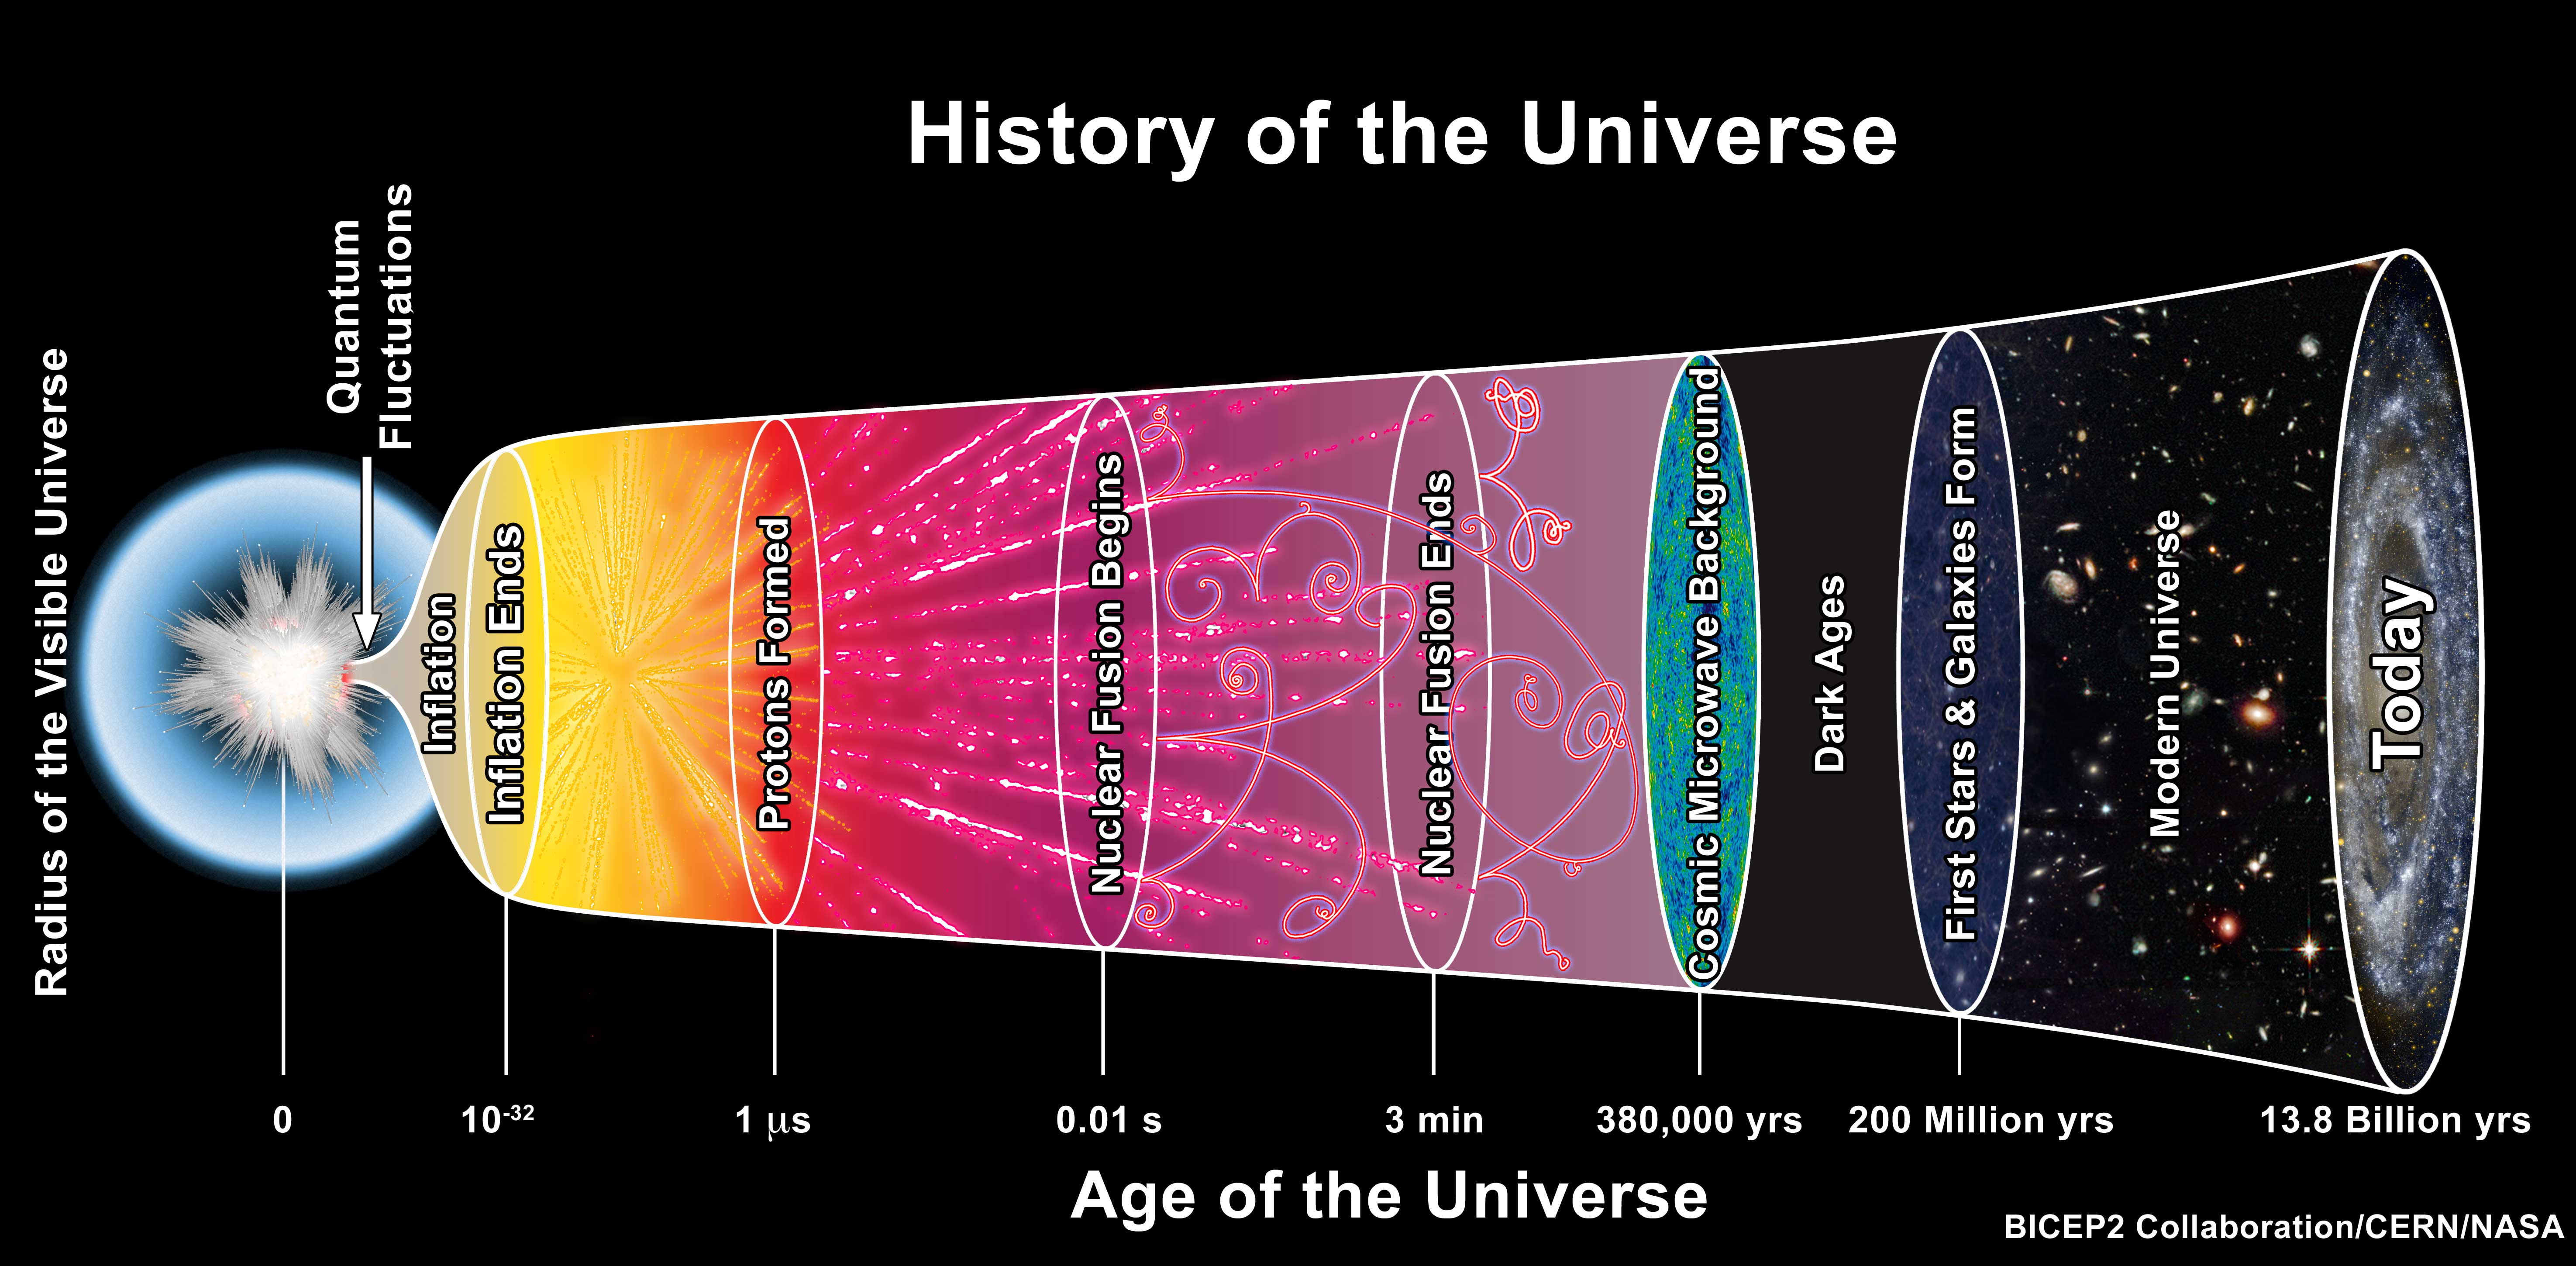
\includegraphics[width=0.8\textwidth]{universe-history}
    \caption{宇宙的演化历史. (来源: BICEP2/CERN/NASA)}
  \end{figure}
\end{frame}

%............
\begin{frame}{研究背景}
  \begin{itemize}
    \item EoR 信号应出现在 $\sim$\,\SIrange{90}{200}{\MHz} 的低频射电波段.
    \item 信号非常微弱,亮温度仅约几 mK 至十几 mK.
    \item 强烈的前景干扰(比 EoR 信号强约 5 个数量级),多种前景干扰成分.
    \item 仪器效应复杂、观测干扰显著、数据处理困难、等等.
    \item 亟待深入理解前景干扰,构建准确的前景模型,
      研发有效的前景处理和 EoR 信号提取算法,
      才能保障 EoR 探测实验的成功.
  \end{itemize}
\end{frame}

%............
\begin{frame}{研究内容}
  \begin{alertblock}{1. 改进射电晕的建模以及评估其对 EoR 探测的影响}
    \begin{itemize}
      \item 星系团射电晕是一类典型的河外射电展源:
        尺度较大(若干角分)、形态相对复杂、
        数目较多(SKA 将发现约 2500 个 \cite{cassano2015}),
        可能对 EoR 信号的探测产生显著干扰.
      \item 相比银河系以及河外点源等前景成分,对射电晕的研究明显不足而且比较粗糙.
      \item 基于\alert{湍流再加速模型},模型星系团的形成与演化过程,
        显著改进射电晕的低频射电天图的模拟.
      \item 采用 \alert{SKA1-Low 阵列布局},整合逼真的干涉阵列仪器效应.
      \item 利用一维和二维功率谱,量化射电晕对 EoR 信号的干扰情况,
        指导 EoR 实验的数据处理以及 EoR 信号分离算法的研发.
    \end{itemize}
  \end{alertblock}
\end{frame}

%............
\begin{frame}{研究内容}
  \begin{alertblock}{2. 基于深度学习研发 EoR 信号分离新算法}
    \begin{itemize}
      \item 传统的前景处理方法依赖于:前景辐射的频谱必须非常光滑.
      \item 干涉阵列的波束存在频率依赖效应,导致前景辐射的频谱出现小尺度涨落,
        光滑性受到损坏.
      \item 波束形状非常复杂,难以为现有方法打造一个实际可用的波束模型.
      \item 深度学习方法能从数据中学习知识并自适应地优化自身模型.
      \item 基于深度学习方法研发 EoR 信号分离新算法更加可行、更具有吸收力.
    \end{itemize}
  \end{alertblock}
\end{frame}



测试 \textbf{测试}\\
空空空空空空空空\\
空\cspace{}空\cspace[2em]{}空

\texttt{code} \textbf{\texttt{code}}

Math:
$E = m c^2$.

X$X$X|x$x$x|M$M$M.

\end{frame}

\begin{frame}{References}
  Some references to showcase [allowframebreaks]
  \cite{li.cdae,li.halo}
\end{frame}

%=====================================================================
\section{总结}

\begin{frame}{结\cspace{}论}
  结论...
\end{frame}

\begin{frame}{已发表论文}
  \small
  \begin{itemize}
    \item
      \textsc{\alert{Li, Weitian}; Xu, Haiguang; Ma, Zhixian; Hu, Dan;
      Zhu, Zhenghao; Shan, Chenxi; Wang, Jingying; Gu, Junhua;
      Zheng, Dongchao; Lian, Xiaoli; Zheng, Qian; Wang, Yu;
      Zhu, Jie; Wu, Xiang-Ping}.
      \enquote{\it Contribution of Radio Halos to the Foreground for
        SKA EoR Experiments,}
      \href{http://adsabs.harvard.edu/abs/arXiv:1905.05399}{%
        2019, ApJ, accepted}
    \item
      \textsc{\alert{Li, Weitian}; Xu, Haiguang; Ma, Zhixian; Zhu, Ruimin;
      Hu, Dan; Zhu, Zhenghao; Gu, Junhua; Shan, Chenxi; Zhu, Jie;
      Wu, Xiang-Ping}.
      \enquote{\it Separating the EoR Signal with a Convolutional Denoising
        Autoencoder: A Deep-learning-based Method,}
      \href{http://adsabs.harvard.edu/abs/2019MNRAS.485.2628L}{%
        2019, MNRAS, 485, 2628}
    \item
      合作论文 12 篇
  \end{itemize}
\end{frame}

\begin{frame}[standout]
  \Huge 谢\cspace{}谢

  \note[item]{感谢导师}
  \note[item]{感谢评审专家}
\end{frame}


%=====================================================================
\appendix

\begin{frame}[standout]
  Appendix
\end{frame}

\begin{frame}[allowframebreaks]{参考文献}
  \printbibliography[heading=none]
\end{frame}

\end{document}
